\documentclass{article}
\usepackage[utf8]{inputenc}
%\author{mo000007 }
\usepackage[left=3cm, right=3cm, top=3cm]{geometry}
\usepackage{graphicx}
\begin{document}

    \begin{titlepage}
      \centering
        \vfill
        {\bfseries\Huge
          PROJECT 3: INTRUDER ALARM \\
            \vskip2cm
          }

          {\bfseries\Large
            IN THIS PROJECT, YOU WILL BUILD MOTION-SENSING ALARM TO DETECT AN INTRUDER USING ULTRASONIC SENSOR, LASER PEN AND PASSIVE INFRARED (PIR) SENSOR\\
          } {

            \vskip1cm
            \today\\
        }
        \vfill
        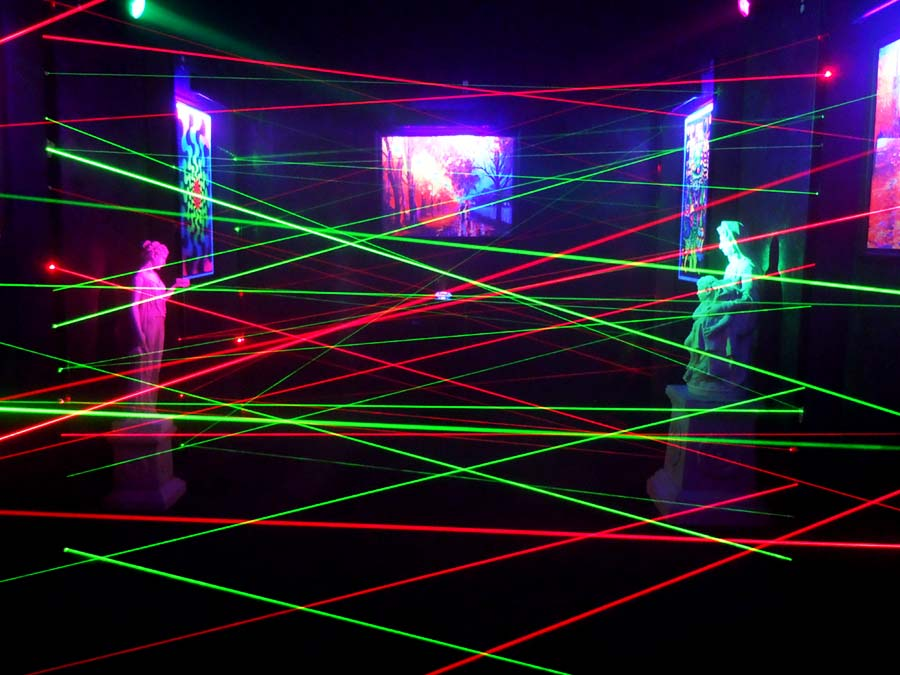
\includegraphics[width=\textwidth]{laser.jpg}
        \vfill
        \vfill
    \end{titlepage}
\newpage

\section{Objectives}\label{sec:objectives}
At the end of this activity, students will be able to:

\begin{itemize}
\item {Intuitively understand the function of the 3 types of motion detection sensors
    commonly employed in home/enterprise security systems.}
\item {Describe situations/scenarios in which one sensor would be preferred over
    another. }
\end{itemize}

\section{Parts Required}\label{sec:parts}

\begin{itemize}
\begin{minipage}{0.4\linewidth}
    \item Arduino board
    \item Breadboard
    \item 4-pin HC-SR04 ultrasonic sensor
    \item Photoresistor
    \item Piezo buzzer
    \item HC SR501 PIR sensor
\end{minipage}
\begin{minipage}{0.4\linewidth}
    \item Servomotor
    \item Jumper wires
    \item Red LED
    \item Green LED
    \item 2 220-ohm resistors
    \item 10k-ohm resistor
\end{minipage}
\end{itemize}

%\begin{center}
%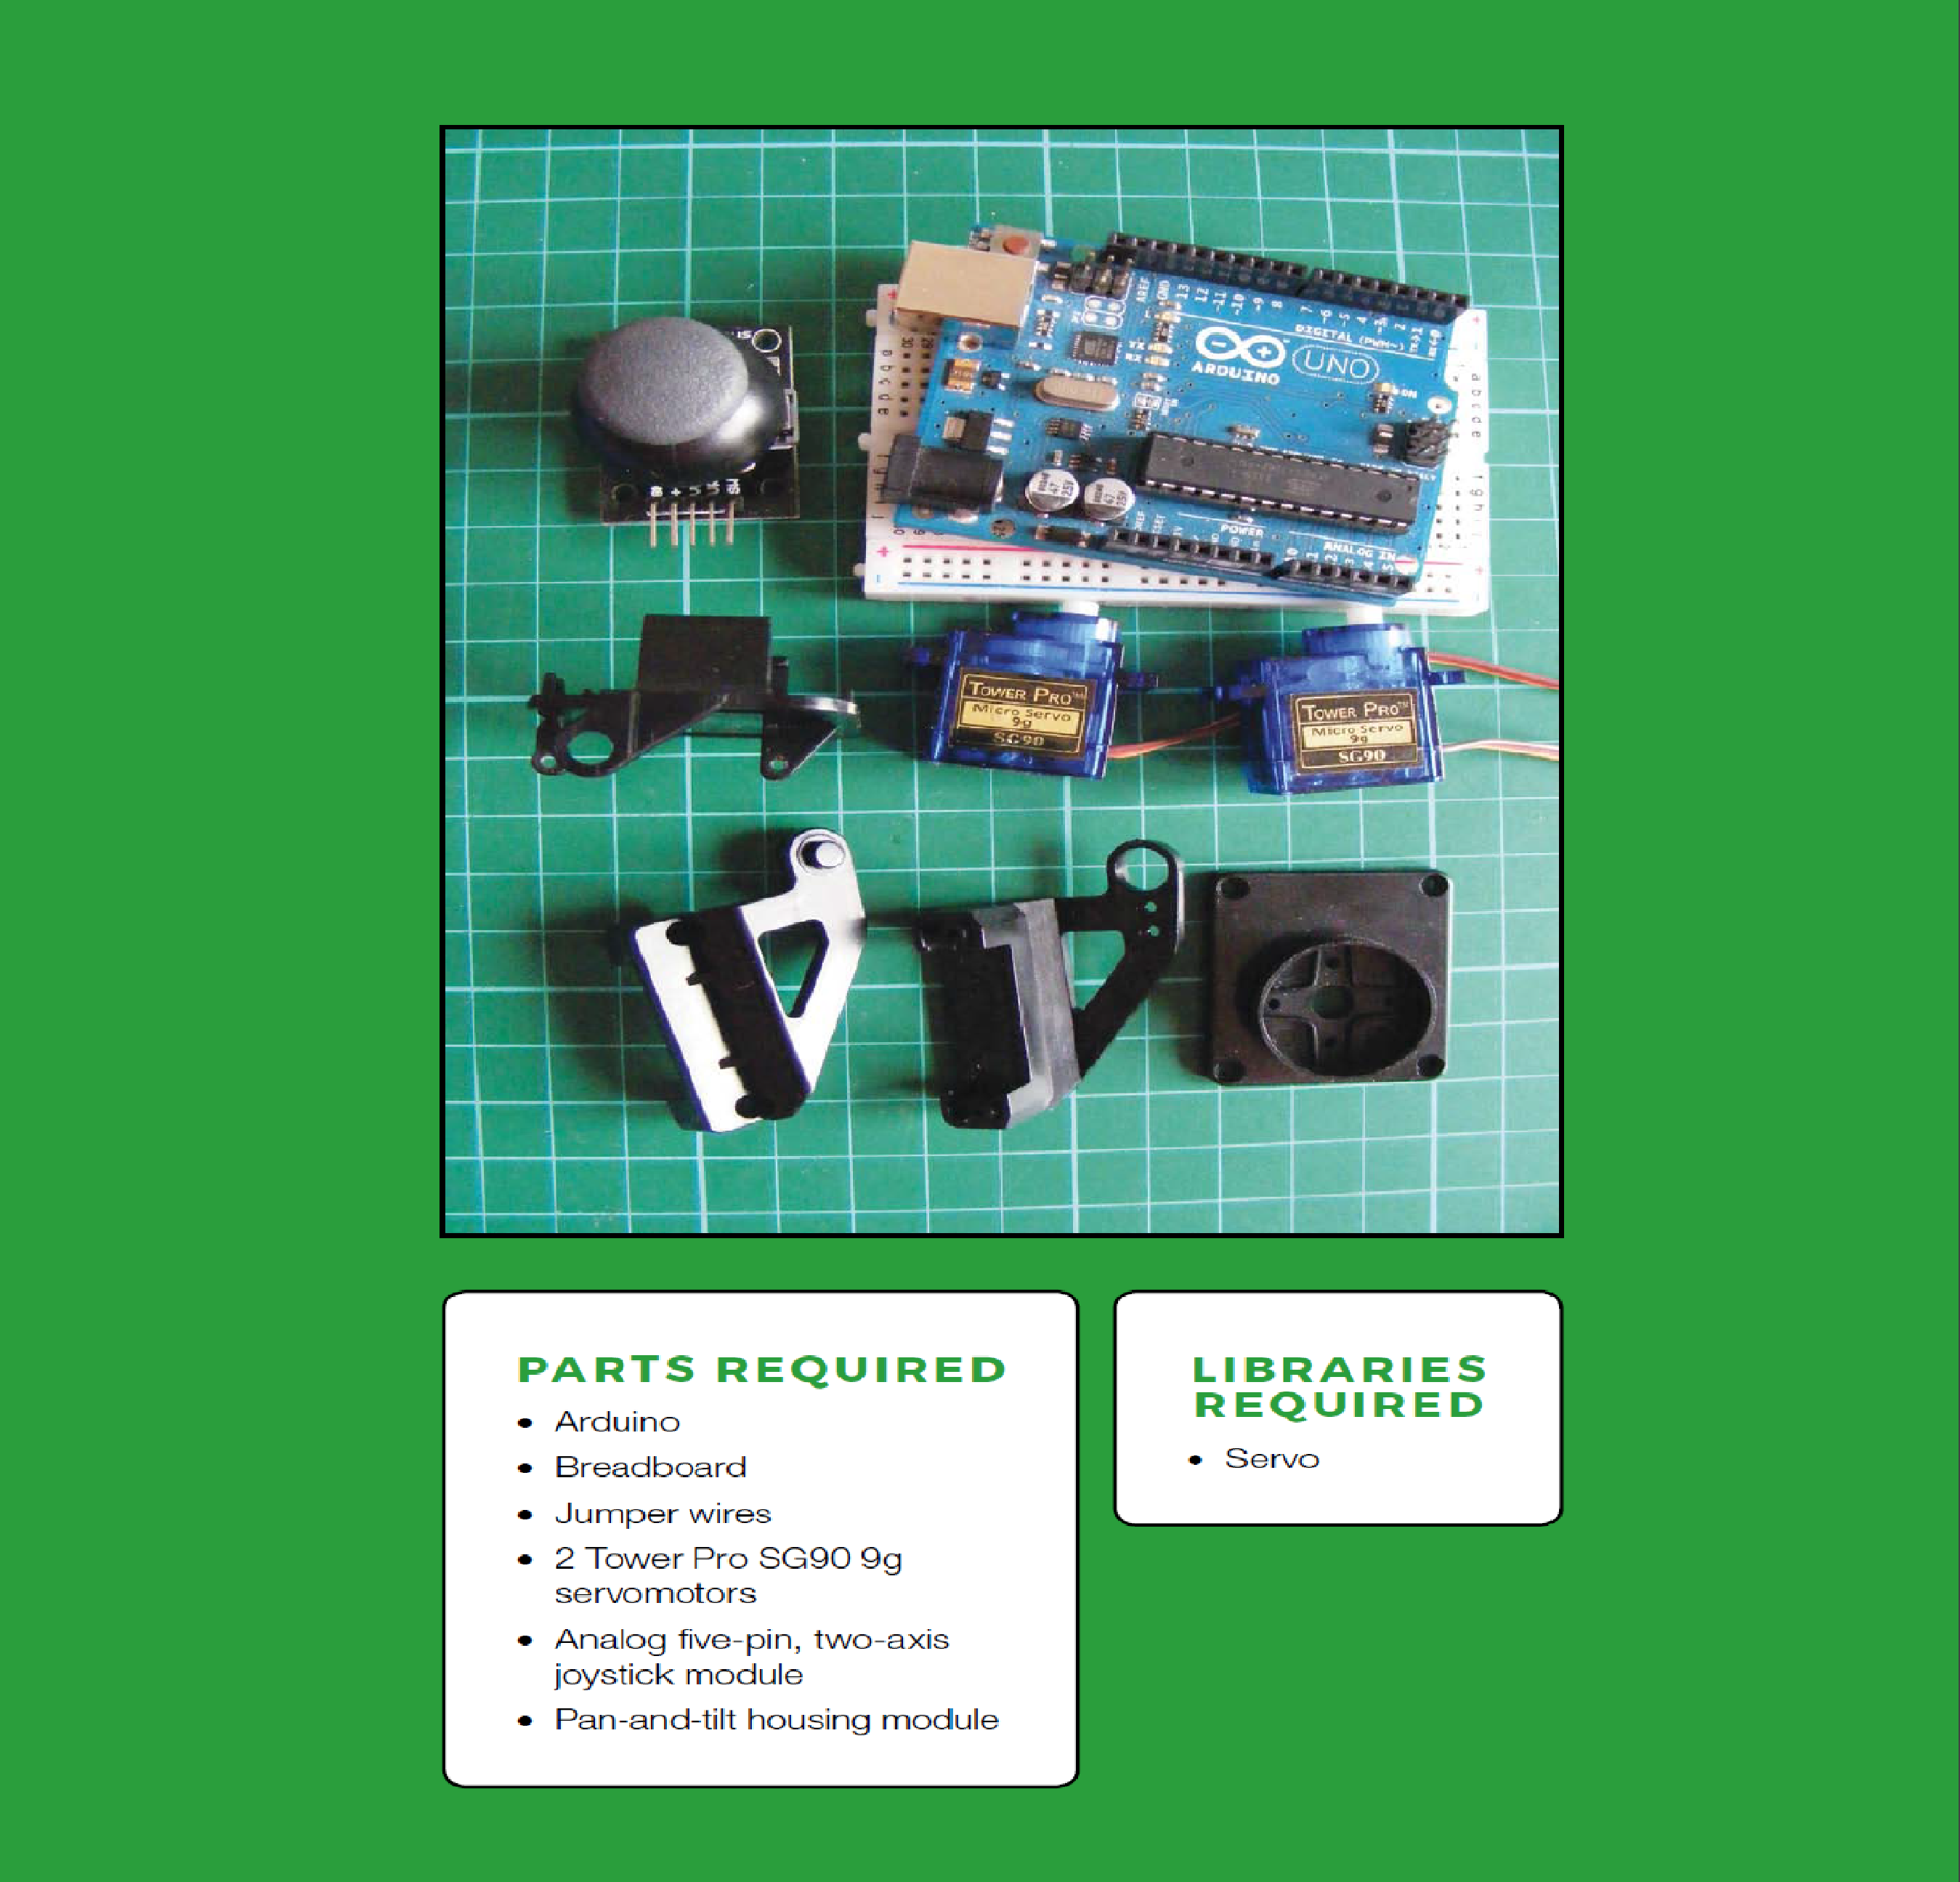
\includegraphics[width=\textwidth, height=18cm]{requir.png}
%\end{center}

\section{Setup}
\begin{enumerate}
\item {Download, unzip, and install the Arduino Integrated Development Environment
    (IDE) from https://www.arduino.cc/en/Main/Donate (does not need admin
    privileges).}
\item {Gather all the necessary parts listed in Sec. \ref{sec:parts}}.
\end{enumerate}

\section{How it Works}
\textbf{Ultrasonic sensor}. Ultrasonic sensors can detect the distance of objects
from them. The sensor works similarly to a radar; it sends out an ultrasonic signal,
or ping. When this signal hits an object, it bounces back like an echo, and the time
between the ping and the echo is used to calculate distance. The Arduino can use this
calculation to trigger an event, depending on the value received. We will use it to
define an area and trigger an alarm when that perimeter is breached (just like you've
seen in the movies!)

\textbf{Photoresistors}. Photoresistors produce variable resistance depending on the
amount of light falling on their sensor. The brighter the light that hits the
resistor, the \emph{lower} the resistance of the circuit and the more current will
flow through it. When the amount of current flowing through the resistor
\emph{increases}, the voltage across the resistor drops (like water flowing over a
dam: the more water is flowing over it, the less pressure is pushing on the
dam). We are going to be shining a laser onto the photoresistor, and if the laser
beam is interrupted, the voltage across it will suddenly \emph{increase}, and the
Arduino will read this increase as tripping our intruder alarm and sound a buzzer.

\textbf{Passive InfraRed (PIR) Sensor}. PIR sensors measure InfraRed (IR) light
radiating from objects in its field of view. They are most often used in PIR-based
motion detectors, like the one we are making, and are good at detecting warm-blooded
moving objects like people moving in its field of view. If something very cold (like
an ice monster) passes in front of it, it will not trigger.


\newpage
\section{Building the Circuits}
In the circuit we are building (Fig. \ref{fig:schematic}), the green LED will be on
when no intruders are detected, and none of the sensors are triggered. When one of
the sensors is triggered:

\begin{enumerate}
\item {The red LED will light up and the green one will turn off.}
\item {The piezo buzzer will beep, simulating an alarm.}
\item {The servo arm will move back and forth, simulating an automated security
    system response.}
\end{enumerate}

We are going to create an intruder detection system with each of the 3 sensors
individually. The schematic is shown for all 3 of the sensors, but you should build
each sensor circuit individually (in whatever order you like!)

\textbf{Which of the 3 sensors is easiest to sneak past? Which is the hardest? Are
  there some situations where one sensor would be better than another?}

\begin{center}
  \label{fig:schematic}
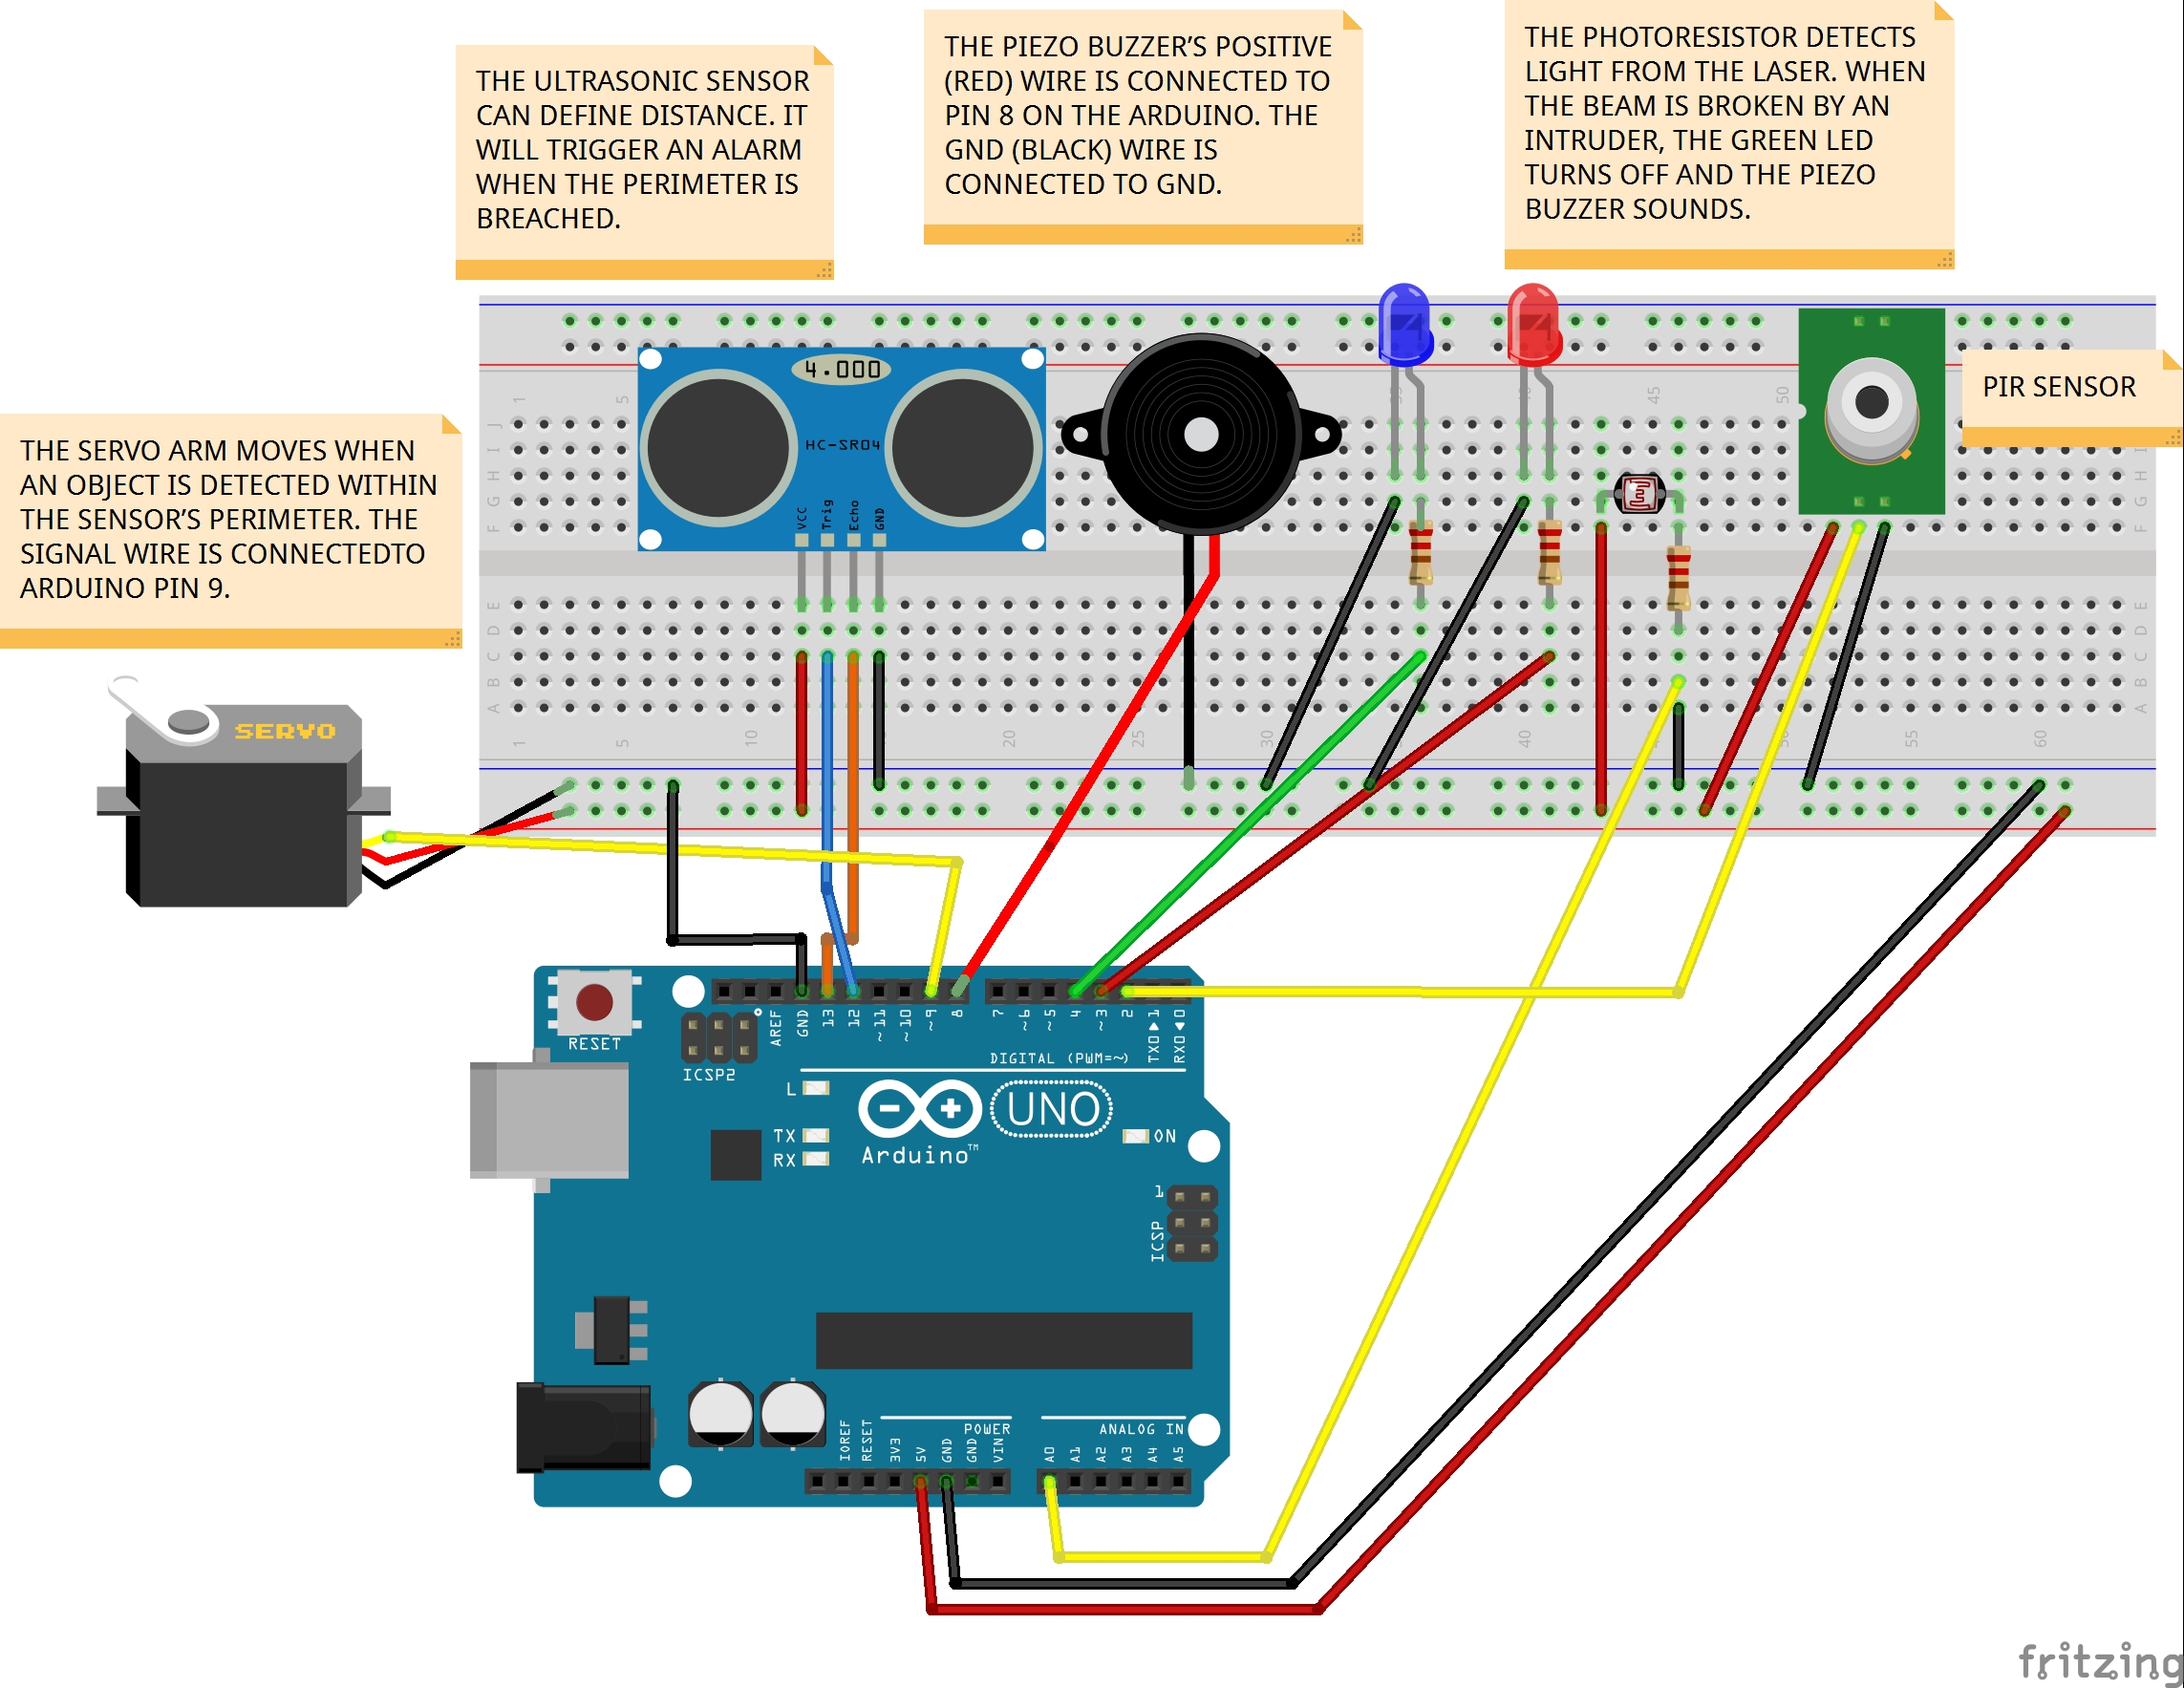
\includegraphics[width=\textwidth]{intruder-alarm.jpg}
\end{center}

% \begin{center}
% \includegraphics[width=6cm]{}
% \end{center}

\section{Programming the Arduino}
The base code for programming the Arduino is provided. Using the Arduino IDE, open
the .ino file.  The IDE allows you to do 4 things: edit the code, verify the code
(i.e. does not contain syntax errors), upload the code to the Arduino, and view the
diagnostic output of things as they run on the Arduino.  Uploading to the Arduino is
easy! Just click the Upload arrow in the IDE.

\section{The Sketch, line by line}
First, we define the pins that each sensor is attached to. The ultrasonic sensor
needs a trigger pin (\verb|US_TRIG_PIN|) and an echo pin (\verb|US_ECHO_PIN|), and
the other two sensors just need trigger pins: \verb|PIR_TRIG_PIN| for the PIR sensor,
and \verb|LASER_TRIG_PIN| for the laser/photoresistor sensor.

In the main \verb|loop()| function, we get the triggered/not triggered state of
whichever sensor we have selected as active via \verb|SECURITY_SENSOR_TYPE|. If the
selected sensor is triggered, then we execute our automated response in
\verb|security_automated_response()|. Otherwise, no intruder is detected and we bring
the servo back to neutral position, and turn the green LED back on and the red one
off (\verb|security_reset()|).

The rest of the code is various helpers to do little pieces of what we have described
above, in order to make things easy to follow.

\section{Extending the Code}
Once you have tried each sensor individually, try to make a more secure system by
employing multiple sensors. Is the resulting system easier or harder to trigger
(sneak past)?

\end{document}
